\chapter{Localization}

In the previous chapters, we have covered the steps to obtain a position of
an object in 2D images. In this chapter, we will take a closer look at
obtaining a position of an object in the world coordinates by combining
information from multiple cameras.

At this point we have computed not only camera parameters for each camera but
also the rotation matrix and the translation vector describing their relative
position. Our goal is to get a position of the object in world coordinates from
a tuple of coordinates from the images taken by cameras.

\section{Projection matrices}
Projection matrices provide a way to transform world coordinates to image
coordinates. The first step is to find out projection matrices for both
cameras, and then we will use them for solving the triangulation problem.

We define a projection matrix as a transformation matrix $P$, such that: $x = P
 X$, where $X$ denotes a vector of size 4$\times$1 -- homogenous world coordinates
of the object and $x$ denotes homogenous object coordinates in the image plane
of the camera -- a vector 3$\times$1.

\subsection{World coordinate system}
We define the world coordinate system as orthogonal, with the origin in the
center of projection of the first (usually left) camera. The positive part of
the z-axis is pointing in front of the camera and below the camera is positive
y-axis and to the right is positive x-axis. Layout and the coordinate system is
displayed in the Figure \ref{fig:coordinate-system}.

\begin{figure}
\centering
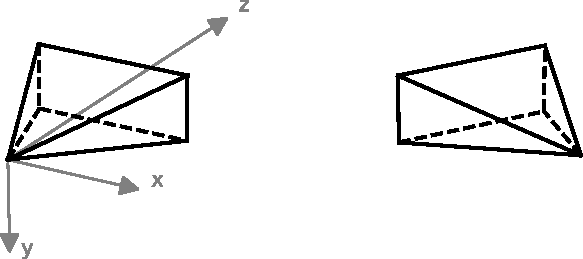
\includegraphics{img/camera-positions}
\caption{Cameras layout and the coordinate system}
\label{fig:coordinate-system}
\end{figure}

\subsection{Computing projection matrices}
After defining coordinate systems, we can compute the projection matrices for
both cameras. We use projection matrix composition to get the projection matrix
from the calibration results.

We compose the projection matrix as $P = K(R|T)$, where $K$ is intristic
camera matrix and $(R|T)$ is extrinsic matrix. $R$ is a rotation matrix and
$T$ is a translation vector. We use this composition to compute the projection
matrices.

\emph{First camera} -- Since we set the origin of the world coordinate system
in the first camera, the camera has no rotation nor translation to the
coordinate system. Therefore we compute the projection matrix as:

\[
 P = K_1 \cdot \begin{pmatrix}
	I_{3, 3} & | & 0_3  
\end{pmatrix}
\]

Where $K_1$ denotes intrinsic parameters matrix of the first camera, $I_{3,3}$ identity
matrix 3$\times$3 and $0_3$ zero vector. Only intristic parameters matrix take
effect on given coordinates, computing from world coordinates in the image plane of the camera.

\emph{Second camera} -- For the second camera's projection matrix, stereo
calibration results will be used. We know the rotation matrix and the
translation vector between the cameras, being able to get coordinates of the
second camera relative to the first one.

We now use this information in construction of the projection matrix, $Q = K_2
\dot (R | T)$, where $K_2$ is intristic parameters matrix of the second camera, $R$
rotation matrix and $T$ translation vector.

More about the decomposition itself can be found in an article by
\citet{computervisionblog}.

%%%%%%%%%%%%%%%%%%%%%%%%%%%

\section{Triangulation}

Now when we know the projection matrices we can formalize our problem as
\begin{equation}
x = PX, y = QX \label{projection-statements}
\end{equation}
with the goal to find $X$. However, errors may occure during
measurement of $x$, $y$ and calibration. In further steps we consider that
calibration results are provided with high accurancy compared to measurement of
$x$ and $y$ (that is the reason to have longer calibration time with more images
at once).

We describe simple linear triangulation, which rewrites the equations
\ref{projection-statements} into format $AX = 0$. A solution for this equation
for unknown $X$ will be the position of the object in world coodinates. This
approach provides a way how to determine four unknowns -- coordinates
of the point $X$ (homogenous).


\subsection{Simple linear triangulation}

We will now shortly describe how the triangulation works under the hood.

We start from the single equation $x = PX$ and try to rearrange it. Since we do
have two such equations (for each camera, see \ref{projection-statements}), we
will create enough equations for finding the unknown position ($X$) of our
object in world coordinates.

We denote a point $x=(a, b, c)$ where $x$ represents homogenous coordinates of
the object in the image. We also choose $a, b, c$ in a way to have $c = 1$. We
can do that, since the coordinates are only up to scale factor.

Then we use the fact, that the cross product of the vector itself is equal to
zero vector. Therefore $x \times PX = 0$ from the previous fact. We rewrite it
to three equations using crossproduct rules:

$$ c(p^{3T}X) - a(p^{2T}X) = 0 $$
$$ b(p^{3T}X) - c(p^{1T}X) = 0 $$
$$ a(p^{2T}X) - b(p^{1T}X) = 0 $$

Where $p^{iT}$ denotes ith row of $P$. Since $c = 1$ we can equally write:

$$ a(p^{3T}X) - (p^{1T}X) = 0 $$
$$ b(p^{3T}X) - (p^{2T}X) = 0 $$
$$ a(p^{2T}X) - b(p^{1T}X) = 0 $$

These equations are linear in the components of $X$. Only two equations are
linearly independent since the third one could be obtained as the sum $b$ times
the first row and $-a$ times the second row. Therefore, we use only the first
two equations

In this way we obtained two equations from $x = PX$. In our case, we have
two such equations -- one for each camera (\ref{projection-statements}). We
denote a point $x = (a, b, 1)$ and $y=(m, n, 1)$. Then using the steps described in previous paragraphs we obtain these equations:

$$ a(p^{3T}X) - (p^{1T}X) = 0 $$
$$ b(p^{3T}X) - (p^{2T}X) = 0 $$
$$ m(q^{3T}X) - (q^{1T}X) = 0 $$
$$ n(q^{3T}X) - (q^{2T}X) = 0 $$

We now can obtain an equation in the form of $AX = 0$. The solution of this
equation is our solution for the position of the object in the worlds
coordinates.

The matrix $A$ has the following format:

\[
A = \begin{pmatrix}
a(p^{3T}) - (p^{1T}) \\
b(p^{3T}) - (p^{2T}) \\
m(q^{3T}) - (q^{1T}) \\
n(q^{3T}) - (q^{2T}) \\
\end{pmatrix}
\]

We can easily check, that multipling the matrix $AX$ gives us the same equation
desribed earlier. Now we analyze what we obtained.

For each image two equations were included, giving a total of four equations in
four homogeneous unknowns.

Without an error during measurements a point $X$ satisfying $AX = 0$ would
exist. However, due to the errors it might not exists. Therefore, a solution to
this equation cannot be find easily. This problem can be solved by direct
linear transformation algorithm (DLT), which will estimate $X$. More about the
method could be found in \citet*{multiple-view-geometry}.

\section*{Implementation note}
For the triangulation we used OpenCV function triangulatePoints($P$, $Q$,
$\mathrm{x}$, $\mathrm{y}$), which is based on simple triangulation method with use of DLT
method for solving equations.
